\section{Quantum query complexity}
\begin{defbox}{: Quantum query computation}
    Given $x \in D$ and a quantum query algorithm $\mathcal{A}$, we write $\mathcal{A}(x)$ for the random variable taking values in $\Gamma$ defined by ($\forall j \in \Gamma$):
    \begin{equation}
        Pr[\mathcal{A}(x) = j] = \norm{\Pi_j U_d(O_x \otimes \II_w)U_{d-1}(O_x \otimes \II_w)\ldots U_1(O_x \otimes \II_w)U_0\ket{0}}^2
    \end{equation}
    Note there are $d+1$ unitaries $U_i$ and $d$ queries to the quantum oracle.

    Let $\e \in (0, 1/2)$, we say $\mathcal{A}$ computes $f$ with bouned error $\e$ if $\forall x \in D$, $Pr[\mathcal{A}(x) = f(x)] \geq 1 - \e$.
\end{defbox}

\begin{figure}[htbp!]
    \centering
    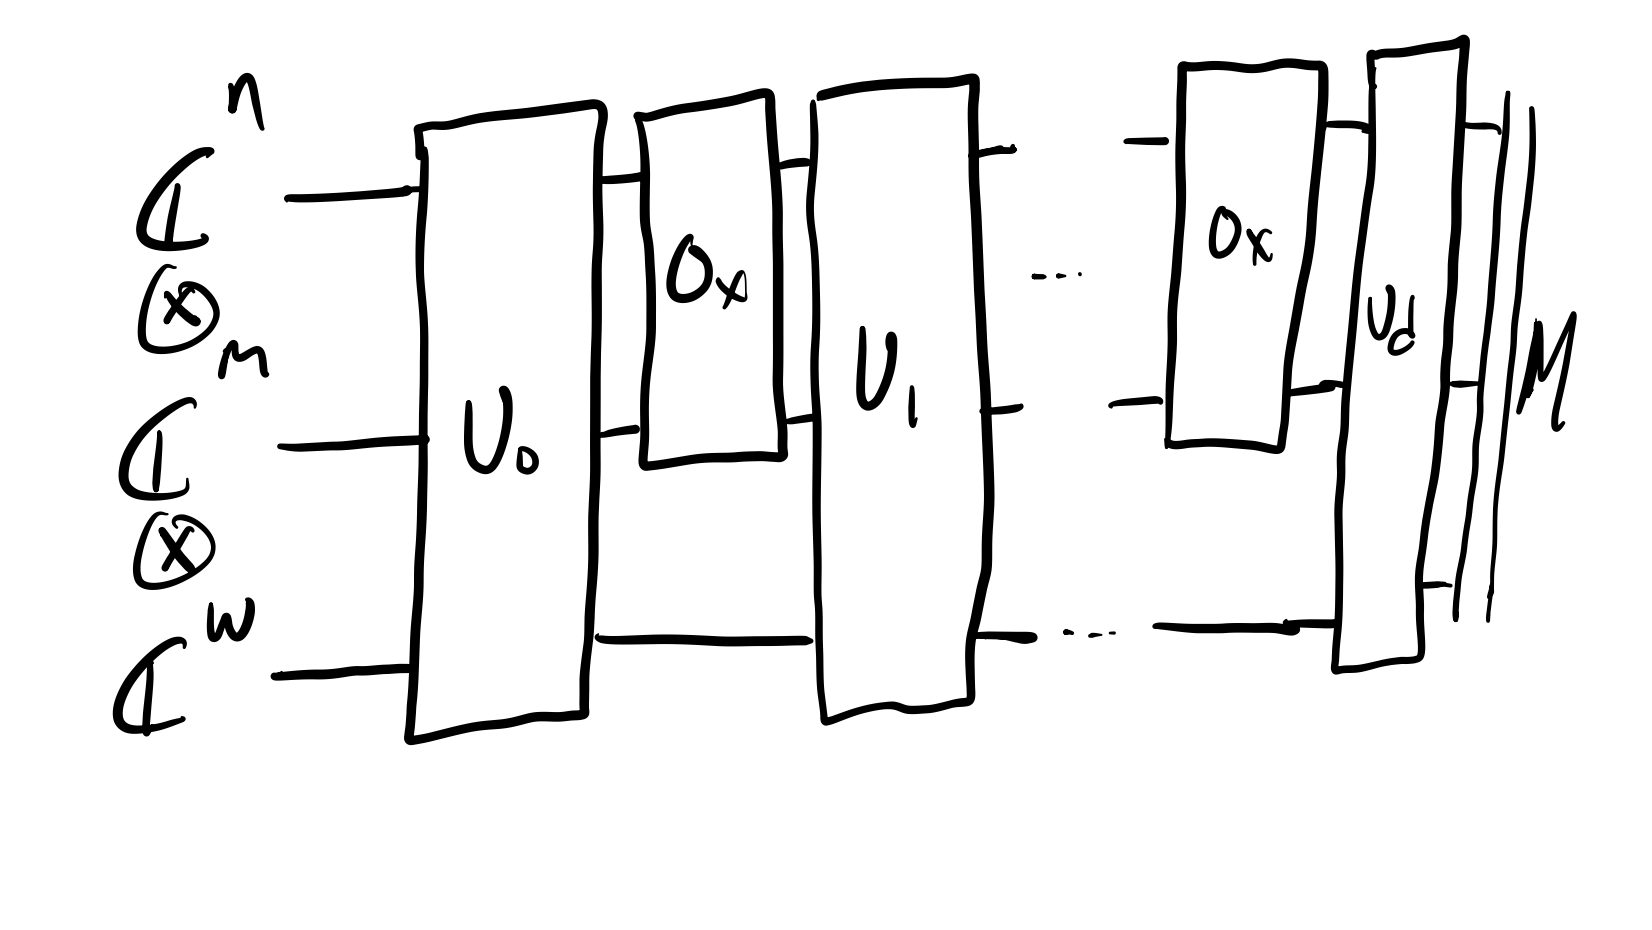
\includegraphics[scale=0.5]{Images/fig-lec3-quantumquerycomp.png}
    \caption{Circuit picture of quantum query computation}
    \label{lec3-quantumquerycomp}
\end{figure}

\begin{defbox}{: Quantum query complexity}
    For $\e \in (0, 1/2)$, $Q_\e(f)$ is defined to be the minimum depth of any quantum query algorithm that computes $f$ with bounded error $\e$. 
\end{defbox}

We now move to the (quantum) Grover algorithm. The upper bound on the quantum query complexity of the Grover algorithm turns out to be $O(\sqrt{n})$, a smaller exponent than the lower bound of the classical query complexity $O(n)$. For $t \in \NN$, consider $OR_n^{o, t}: \set{x \in \set{0, 1}^n \vert \abs{x} = 0 \text{ or } \abs{x} = t} \to \set{0, 1}$. 

\begin{propbox}{: Grover's Algorithm}
    For all $n \in \NN$, $t \in \NN$ such that $t \leq \frac{n}{3}$, we have $Q(OR_n^{0, t}) \leq \frac{\pi}{4}\sqrt{\frac{n}{t}}$. 
\end{propbox}

\begin{defbox}{: Quantum phase oracle}
    For $x \in \set{0, 1}^n$, the quantum phase oracle of $x$ is the unitary matrix $U_x \in \CC^{2n \times 2n}$ defined by:
    \begin{equation}
        U_x\ket{i}\ket{b} = (-1)^{x_{i+1}b}\ket{i}\ket{b}
    \end{equation}
    where $i \in \set{0, 1, \ldots, n-1}$ and $b \in \set{0, 1}$. 
\end{defbox}

\begin{lembox}{: Phase kickback trick}
    For all $x \in \set{0, 1}^n$:
    \begin{equation}
        U_x = (\II_n \otimes H)O_x(\II_n \otimes H)
    \end{equation}
    where $H = \frac{1}{\sqrt{2}}\m{1 & 1 \\ 1 & -1}$. 
\end{lembox}
\begin{proof}
    First, notice that for $b \in \set{0, 1}$, we have:
    \begin{equation}
        H\ket{b} = \frac{1}{\sqrt{2}}(\ket{0} + (-1)^b\ket{1})
    \end{equation}

    Then, it suffices to show that $\text{RHS}\ket{i}\ket{b} = \text{LHS}\ket{i}\ket{b}$. We have:
    \begin{align*}
        \text{RHS}\ket{i}\ket{b} &= (\II_n \otimes H)O_x\ket{i}H\ket{b} 
        \\ &= (\II_n \otimes H)O_x\ket{i}\frac{1}{\sqrt{2}}(\ket{0} + (-1)^b\ket{1})
        \\ &= \frac{1}{\sqrt{2}}(\II_n \otimes H)(\ket{i}\ket{x_{i+1}} + \ket{i}(-1)^b\ket{1 \oplus x_{i+1}})
        \\ &= \frac{1}{\sqrt{2}}\left(\ket{i}\frac{1}{\sqrt{2}}(\ket{0} + (-1)^{x_{i+1}}\ket{1}) + \ket{i}\frac{1}{\sqrt{2}}(\ket{0} + (-1)^{x_{i+1} \oplus 1}\ket{1})(-1)^b\right)
        \\ &= \frac{1}{2}\ket{i}\left((1 + (-1)^b)\ket{0} + ((-1)^{x_{i+1}} - (-1)^b(-1)^{x_{i+1}})\ket{1}\right)
        \\ &= \begin{cases}
            \ket{i}\ket{0} & b = 0
            \\ (-1)^{x_{i+1}}\ket{1} & b = 1
        \end{cases}
        \\ &= (-1)^{bx_{i+1}}\ket{i}\ket{b}
    \end{align*}
\end{proof}

A quick note - $H$ is unitary, hence invertible - in fact $H^\dag = H^{-1} = H$ so $H^2 = \II_2$ and as a result we find that:
\begin{equation}
    O_x = (\II_n \otimes H)U_x(\II_n \otimes H)
\end{equation}

The quantum query complexity only cares about calls to the oracle $O_x$. So, the query complexity does not change if we change the oracle to the phase oracle (the difference can be absorbed into the sequence $U_0, \ldots U_d$).

We now prove the Grover proposition.

\begin{proof}
    Let $\ket{\psi}$ denote the $n$-dimensional state:
    \begin{equation}
        \ket{\psi} = \frac{1}{\sqrt{n}}\sum_{i=0}^{n-1}\ket{i}.
    \end{equation}
    For $x \in \set{0, 1}^n$, let $V_x \in \CC^{n \times n}$ be:
    \begin{equation}
        V_x\coloneqq \sum_{i=0}^{n-1}(-1)^{x_{i+1}}\dyad{i}{i} = \II_n - 2\sum_{i\vert x_{i+1} = 1}\dyad{i}{i}
    \end{equation}
    Side note; if $b = 1$ then, $U_x\ket{i}{b} = (-1)^{x_{i+1}b}\ket{i}\ket{b} = (-1)^{x_{i+1}}\ket{i}\ket{1}$. 
    Define $G \in \CC^{n \times n}$ as:
    \begin{equation}
        G \coloneqq \II_n - 2\dyad{\psi}{\psi}.
    \end{equation}
    Finally, let:
    \begin{equation}
        \Pi_0 \coloneqq \dyad{\psi}{\psi}.
    \end{equation}
    Our measurement is $\mathcal{M} \coloneqq \set{\Pi_0, \II_n - \Pi_0}$. Then for $k \in \NN$, consider:
    \begin{equation}
        p_x \coloneqq \norm{\Pi_0(GU_x)^k\ket{\psi}}^2
    \end{equation}
    This can be thought as the probability that a $k$-query quantum algorithm outputs zero. In this setting $U_0$ is the unitary such that $U_0\ket{0}^n = \ket{\psi}$, and $U_1, \ldots U_k = G$. 

    There are two cases. We have restricted the domain of the $OR$ to be Hamming weight $0$ (i.e. $O^n$) and with Hamming weight $t$.
    \begin{enumerate}
        \item If $x = 0^n$, then $V_x = \II_n$, $G = 1 - 2\dyad{\psi}{\psi}$. Then:
        \begin{equation}
            (GV_x)\ket{\psi} = G\ket{\psi} (\II_n - 2\dyad{\psi}{\psi})\ket{\psi} = \ket{\psi} - 2\ket{\psi} = -\ket{\psi} \implies (GV_x)^k\ket{\psi} = (-1)^k\ket{\psi}
        \end{equation}
        and so $p_x = \norm{\dyad{\psi}{\psi}(-1)^k\ket{\psi}}^2 = 1$. 
        \item If $x$ has Hamming weight $t$, then define:
        \begin{equation}
            \ket{\psi_0} = \frac{1}{\sqrt{n-t}}\sum_{i\vert x_{i+1} = 0}\ket{i}, \quad  \ket{\psi_1} = \frac{1}{\sqrt{t}}\sum_{i\vert x_{i+1} = 1}\ket{i}
        \end{equation}
        Then, by inspection:
        \begin{equation}
            \ket{\psi} = \sqrt{1-\frac{t}{n}}\ket{\psi_0} + \sqrt{\frac{t}{n}}\ket{\psi_1} = \cos\vartheta\ket{\psi_0} + \sin\vartheta\ket{\psi_1}
        \end{equation}
        where $\vartheta \coloneqq \arcsin(\sqrt{t/n}) \in [0,\pi/2]$. We have:
        \begin{equation}
            GV_x\ket{\psi_0} = G\ket{\psi_0} = \ket{\psi_0} - 2\ket{\psi}\braket{\psi}{\psi_0} = \ket{\psi_0} - 2\cos\vartheta\ket{\psi} = -\cos2\vartheta\ket{\psi_0} - \sin2\vartheta\ket{\psi_1}
        \end{equation}
        \begin{equation}
            GV_x\ket{\psi_1} = -G\ket{\psi_1} = -\sin(2\vartheta)\ket{\psi_0} -\cos(2\vartheta)\ket{\psi_1}
        \end{equation}
        So - we can analyze the entire algorithm in the 2-dimensional subspace spanned by $\ket{\psi_0}, \ket{\psi_1}$ (which we note are orthogonal). Within the subspace $\text{span}\set{\ket{\psi_0}, \ket{\psi_1}}$, we can write $GV_x$ as:
        \begin{equation}
            -GV_x \cong \m{\cos(2\vartheta) & -\sin(2\vartheta) \\ \sin(2\vartheta) & \cos(2\vartheta)}
        \end{equation}
        We then have (informally by composition of rotations - formally via diagonalization):
        \begin{equation}
            (-GV_x)^k = \m{\cos(2k\vartheta) & -\sin(2k\vartheta) \\ \sin(2k\vartheta) & \cos(2k\vartheta)}
        \end{equation}
        Therefore:
        \begin{equation}
            (GV_x)^k\ket{\psi} = (-1)^k\left(\cos((2k+1)\vartheta)\ket{\psi_0} + \sin((2k+1)\vartheta)\ket{\psi_1}\right)
        \end{equation}
        and so:
        \begin{equation}
            p_x = \norm{\Pi_0(GV_x)^k\ket{\psi}}^2 = \cos^2(2k\vartheta)
        \end{equation}
        $k$ is the number of queries, so what do we choose? We choose it such that we can distinguish it from the all $0$ case. I.e. that $p_x = 0$ and so $k = \frac{\pi}{4\vartheta}$. $\vartheta = \arcsin(\sqrt{t/n}) \sim \sqrt{t/n}$ so we choose $k = \frac{\pi}{4}\sqrt{\frac{n}{t}}$. 
    \end{enumerate}
\end{proof}